\documentclass[12pt,a4paper]{article}
\usepackage[utf8]{inputenc}
\usepackage[polish]{babel}
\usepackage[T1]{fontenc}
\usepackage{graphicx}
\usepackage{geometry}
\usepackage{caption}
\usepackage{subcaption}
\usepackage{booktabs}   % Podstawa: \toprule, \midru    le, \bottomrule
\usepackage{multirow}   % Do łączenia wierszy
\usepackage{siunitx}    % Do wyrównywania liczb względem kropki dziesiętnej

\geometry{margin=1in}

\title{Raport z Laboratorium 1}
\author{Kajetan Frąckowiak}
\date{\today}

\begin{document}

\maketitle

\section{Punkt 1 i 3}

W ramach ćwiczenia przeprowadzono analizę procesu uczenia modeli typu MLP (Multilayer Perceptron) o różnych architekturach i liczbie epok. Poniżej przedstawiono wyniki w postaci krzywych strat oraz uzyskanej dokładności (accuracy) na zbiorze testowym.

\begin{figure}[htbp]
     \centering
     \begin{subfigure}[b]{0.48\textwidth}
         \centering
         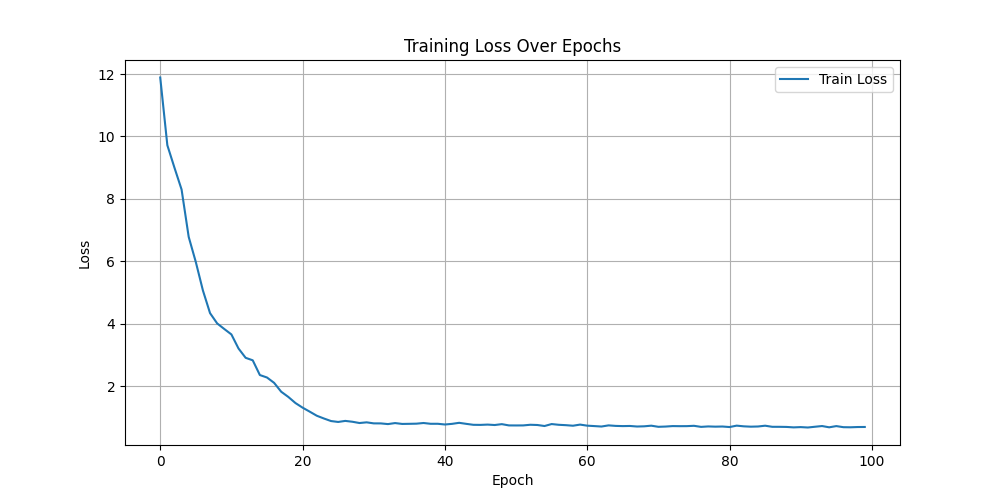
\includegraphics[width=\textwidth]{../src/plots/loss_curve_v1_100.png}
         \caption{100 epok}
         \label{fig:loss_v1_100}
     \end{subfigure}
     \hfill
     \begin{subfigure}[b]{0.48\textwidth}
         \centering
         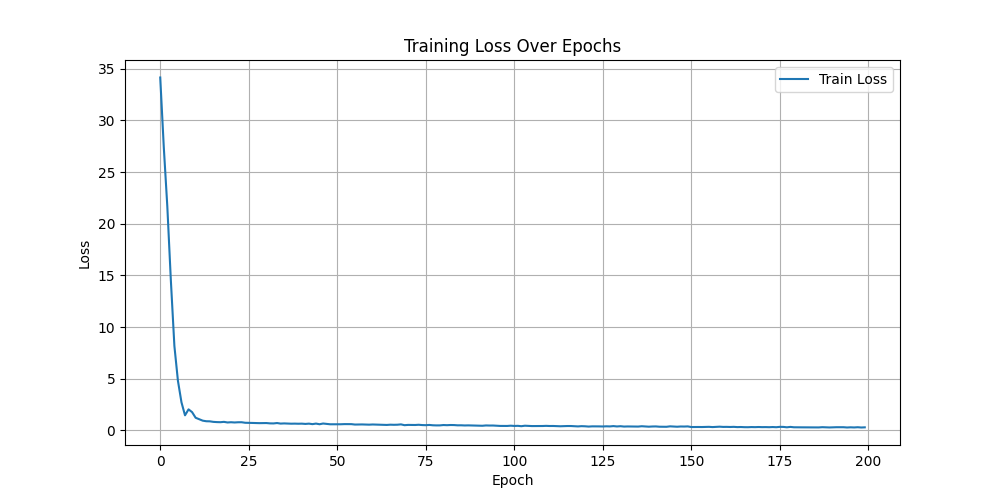
\includegraphics[width=\textwidth]{../src/plots/loss_curve_v1_200.png}
         \caption{200 epok}
         \label{fig:loss_v1_200}
     \end{subfigure}
     \caption{Krzywe strat dla modelu MLP z 1 warstwą ukrytą (16 neuronów). Wyraźny wzrost dokładności przy wydłużeniu czasu uczenia.}
     \label{fig:v1_comparison}
\end{figure}

\begin{figure}[htbp]
     \centering
     \begin{subfigure}[b]{0.48\textwidth}
         \centering
         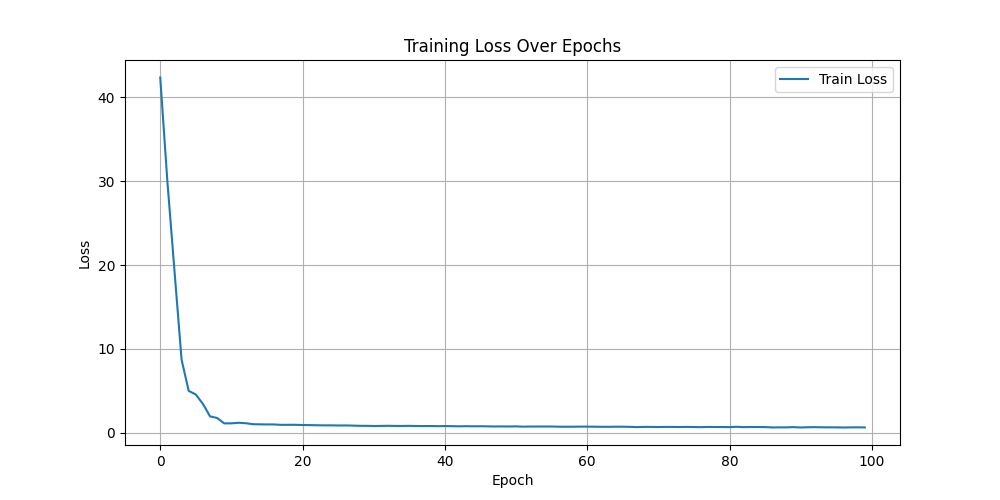
\includegraphics[width=\textwidth]{../src/plots/loss_curve_v2_100.png}
         \caption{100 epok}
         \label{fig:loss_v2_100}
     \end{subfigure}
     \hfill
     \begin{subfigure}[b]{0.48\textwidth}
         \centering
         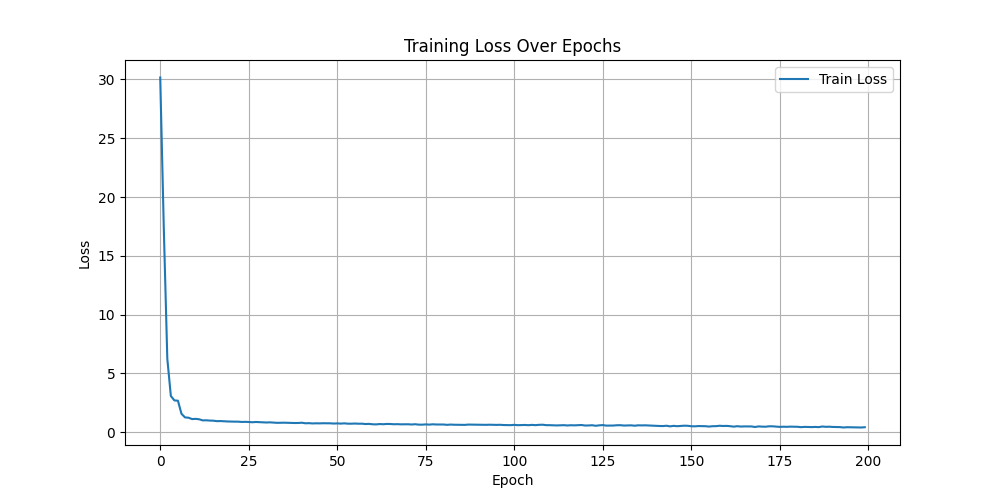
\includegraphics[width=\textwidth]{../src/plots/loss_curve_v2_200.png}
         \caption{200 epok}
         \label{fig:loss_v2_200}
     \end{subfigure}
     \caption{Krzywe strat dla modelu MLP z 2 warstwami ukrytymi (32 i 16 neuronów). Widoczna fluktuacja straty przy 200 epokach sugerująca potencjalny overfitting.}
     \label{fig:v2_comparison}
\end{figure}

\begin{table}[t] % 't' oznacza top - standard w publikacjach
\centering
\caption{\textbf{Porównanie wydajności modeli.} Wyniki accuracy dla różnych architektur MLP oraz algorytmu k-NN na zbiorze testowym. Pogrubiono najlepsze wyniki.}
\label{tab:results}
\vspace{2mm} % Lekki odstęp pod podpisem
\begin{tabular}{llcc}
\toprule
\textbf{Model} & \textbf{Konfiguracja} & \textbf{Epoki} & \textbf{Accuracy (\%)} \\
\midrule
k-NN & $k=1$ & -- & \textbf{100.0} \\
k-NN & $k=3$ & -- & 87.08 \\
k-NN & $k=5$ & -- & 78.7 \\
k-NN & $k=10$ & -- & 79.21 \\
\midrule
MLP (1-layer) & 16 units & 100 & 75.0 \\
              & 16 units & 200 & 94.4 \\
\addlinespace % Delikatny odstęp zamiast linii
MLP (2-layer) & 32--16 units & 100 & 91.6 \\
              & 32--16 units & 200 & 88.8 \\
\bottomrule
\end{tabular}
\end{table}

Jak widać w tablicy 1, model k-NN (k = 1) wykazał najlepszą dokładność ze wszystkich modeli, co jest zrozumiałe dla małych zbiorów danych jak WINE. A modeli parametrycznych najlszą dokładnością wykazał sie model MLP (1-layer) 16 units który był trenowany na 200 epokach. Jak widzimy na rysunkach 1 i 2 wszystkie modele po
15-25 epoce zaczynają dochodzić do starty równej 0 co ozncza, że nie warto uczyć modelu na bardzo wielu epokach na tak małych zbiorach danych jeżeli nie zależy nam nam na zmiejszaniu strat do paru miejsc po przecinku. Rysunki także pokazają, że modele z wiekszą liczbą parametrów trenowalnych szybciej dochodziły do straty bliskiej zeru, co oznacza, że można wybrać pomiędzy 
mniejszą liczbą neuronów i większą liczbą epok lub mniejszą liczbą epok i większą liczbą neuronów na tak małym zbiorze danych jak WINE.

\section{Punkt 2}
\subsection{Dlaczego skalowanie jest konieczne?}
Skalowanie parametrów modelu jest koniczne by zwiększać dokładność, lecz gdy zwiększamy liczbę parametrów powinniśmy też często większyć liczbę danych treningowych.
\subsection{Co się stanie, jeśli usuniemy jedną warstwę?}
Usunięcie jednej warstwy ukrytej z modelu MLP spowoduje zmniejszenie jego zdolności do modelowania złożonych zależności w danych. Model stanie się prostszy, co może prowadzić do gorszej dokładności, zwłaszcza jeśli dane są nieliniowe. W przypadku bardzo prostych danych, model bez warstwy ukrytej może nadal osiągać dobre wyniki, ale w większości przypadków będzie to prowadzić do spadku wydajności.
\subsection{Jak zmiana learning rate wpływa na zbieżność?}
Celem uczenia modelu ML jest dojście do minimów funkcji celu. Jeżeli ustawimy szybko zbyt duży learning rate możemy stale przeskakiwać wraz z gradientem nad minimum, co spowoduje, że model nigdy nie dojście do konwergencji.
Z kolei zbyt mały learning rate może spowodować do bardzo szybkiego wejścia w słabe lokalne optimum z którego nigdy nie wyjdzie. Dlatego zalecane jest stopniowe zmiejszane learning rate wraz z epokami uczenia.
\end{document}